\documentclass[a4paper, 10pt]{article}
\usepackage[spanish] {babel}
\title{Trabajo Practico 3}
\usepackage{floatflt}
\usepackage{tporga2}
\usepackage{caratula}
\usepackage[pdftex]{graphicx}
\usepackage{color}

\setlength{\leftmargin}{2cm}
\setlength{\rightmargin}{2cm}
\setlength{\oddsidemargin}{-1cm}
\setlength{\evensidemargin}{-1cm}
\setlength{\topmargin}{-1cm}
\setlength{\textwidth}{18cm}
\setlength{\textheight}{25cm}

\usepackage{fancyhdr}
\pagestyle{fancy}
\fancyhf{}
\fancyhead [LO,LE]{\scriptsize Trabajo Pr\'actico N$^{\circ}$3}
\fancyhead [RO,RE]{\scriptsize Gonzales, Mancuso, Mataloni}
\fancyfoot[CE,CO]{\thepage}
\renewcommand{\footrulewidth}{0.4pt}

\usepackage[pdftex, bookmarks=true, colorlinks, citecolor=black, linkcolor=black]{hyperref}
\usepackage{multirow}
\usepackage{listings}

\begin{document}


\materia{Organizaci\'on del Computador II}
\submateria{Segundo Cuatrimestre de 2009}
\titulo{Trabajo Practico N$^{\circ}$3}
\grupo{Grupo RET}
\integrante{Gonzales Courtois Matias}{453/07}{curtu\_infinito73@hotmail.com}
\integrante{Mancuso Emiliano}{597/07}{emiliano.mancuso@gmail.com}
\integrante{Mataloni Alejandro}{706/07}{amataloni@gmail.com}
\maketitle
\newpage

\addcontentsline{toc}{section}{\'Indice}
\tableofcontents

\newpage

\section{Ejercicio 1}

\subsection{Completar Tabla Descriptores Globales}

Para realizar \'este ejercicio no utilizamos los archivos gdt.h y gdt.c sino que completamos la tabla global de descriptores \texttt{GDT} en el \texttt{kernel.asm}. 
\'Esta fue la soluci\'on al siguiente problema \\ \\
\centerline{ \texttt{relocation truncated to fit: R\_386\_16 against `GDT\_DESC'}} \\ 

 Lo primero que tuvimos que hacer fue posicionarnos en la direcci\'on de memoria en la cual debe estar la \texttt{GDT}. Como en el enunciado del TP nos ped\'ia que la \texttt{GDT} est\'e en la direcci\'on de memoria 0xE000, al final de nuestro archivo Kernel.asm y luego de la definici\'on de las cosas que nos piden en ejercicios posteriores escribimos la siguiente linea:

\lstset{language=[x86masm]Assembler}
\begin{lstlisting}
			TIMES 0xE000 - KORG - ($ - $$) db 0x00 
\end{lstlisting} 
\texttt{Instrucci\'on para llenar de ceros hasta la direcci\'on 0xE000}. \\
\texttt{TIMES:} Funci\'on del nasm que repite el c\'odigo. \\

Como ya estabamos en la direcci\'on correcta comenzamos a llenar la \texttt{GDT} de la siguiente manera:
 
\lstset{language=[x86masm]Assembler}
\begin{lstlisting}
ALIGN 0x10
gdt:
;descriptor nulo
	dd 0x00	
	dd 0x00
	
; 0x8 (1) descriptor segmento de codigo
	dw 0xffff	; segment limit
	dw 0x00		; base 15
	db 0x00		; base
	db 10011010b	; p(1)|dpl(2)|s(1)|type(4)
	db 11001111b 	; g(1)|db(1)|l(1)|avl(1)|seglim(4)
	db 0x00		; base 31:24
	 
; 0x10(2) descriptor segmento de datos
	dw 0xffff	; segment limit
	dw 0x00		; base 15
	db 0x00		; base
	db 10010010b	; p(1)|dpl(2)|s(1)|type(4)
	db 11001111b 	; g(1)|db(1)|l(1)|avl(1)|seglim(4)
	db 0x00		; base 31:24 
	
; 0x18(3) descriptor segmento de video
	dw 0xffff	; segment limit
	dw 0x8000	; base 15
	db 0x0B		; base
	db 10010010b	; p(1)|dpl(2)|s(1)|type(4)
	db 11001111b 	; g(1)|db(1)|l(1)|avl(1)|seglim(4)
	db 0x00		; base 31:24
	
	gdt_descriptor:
	dw gdt_end - gdt
	dd gdt 
	
\end{lstlisting}

\newpage

Primero definimos un segmento nulo, luego el segmento de codigo con los respectivos atributos que ocupa toda la memoria, luego el segmento de datos solapado con el de codigo, y por ulimo el segmento que direcciona a la memoria de video.

\subsection{Pasar a modo protegido}

Para pasar a modo protegido primero debemos setear algunas cosas. En principio debemos habilitar la \texttt{gate A20} la cual nos permite direccionar m\'as de 1 Mb. Luego tenemos que setear 
la informaci\'on (direcci\'on y limite) de la GDT en el registro \texttt{gdtr}. Una vez realizados estos pasos debemos setear el bit que habilita la paginaci\'on en el registro \texttt{CR0}. Luego hacemos un \texttt{jump} con el descriptor de segmento de c\'odigo.

\lstset{language=[x86masm]Assembler}
\begin{lstlisting}
	;Habilitar Gate 20
	call enable_A20
	
	;Cargar el registro GDTR
	lgdt [gdt_descriptor]	; cargamos la gdt
		
	;Pasar a modo protegido
	mov eax, cr0
	or eax, 1
	mov cr0, eax
	jmp 0x08:modoprotegido
\end{lstlisting}

\subsection{Pintar marco}
Para pintar el marco, seteamos los registros de segmento con el n\'umero correspondiente (en nuestro caso 0x18) para utilizar el segmento de la memoria de video. \\
Una vez hecho esto utilizamos una serie de ciclos para escribir lo que nosotros quer\'iamos, utilizando contadores y mensajes definidos.

\begin{center}
	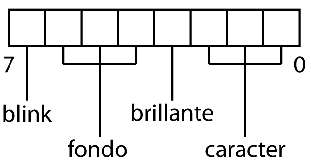
\includegraphics[scale=0.60]{Graficos/word_video.png}
\end{center}
\texttt{Cada elemento es de 2 bytes. Primero es el Modo, luego el caracter ASCII}. 
 
\newpage
  
\section{Ejercicio 2}
\subsection{ Inicializar directorios y tablas de p\'aginas }

Al igual que en el ejercicio \texttt{1.1}, para inicializar los directorios y tablas de p\'aginas nos posicionamos en la direcci\'on de memoria correspondiente seg\'un la tarea.

\vspace*{2em}

\begin{center}
	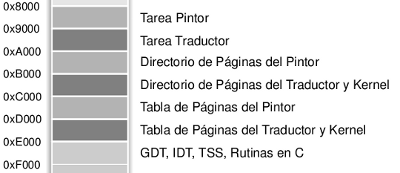
\includegraphics[scale=0.65]{Graficos/directorios_y_tablas_de_paginas.png}
\end{center}

\vspace*{2em}

Tanto el directorio de p\'aginas del \texttt{Pintor} (direcci\'on 0xA000 a 0xAFFF) como el del \texttt{Traductor} (direcci\'on 0xB000 a 0xBFFF) lo llenamos completamente (4kb), con descriptores de tablas de p\'aginas caracterizados como: \\ \\
\centerline{\textit{ supervisor, read/write, not present} \texttt{(0x00000002)}} \\

A su vez, para crear los descriptores de p\'agina en cada tabla, procedemos de la misma manera que los directorios de p\'aginas.

Para el \texttt{Pintor} necesitamos hacer \texttt{identity mapping} de las direcciones:
\begin{itemize}
	\item 0x0000  a 0x8FFF
	\item 0xE000  a 0xFFFF
	\item 0x15000 a 0x15FFF
\end{itemize}

\lstset{language=[x86masm]Assembler}
\begin{lstlisting}
	;llenamos la primer tabla.
	;pintorTable es la direccion de la primer tabla del pintor
	mov 	esi,pintorTable		
	mov 	eax, 0
	mov ecx,9 						
	  ;Desde 0x0000 hasta 0x8FFF
	llenarTablas:
		or 	eax, 0x3				
		   ; supervisor, read/write, present
		mov 	[esi], eax
		lea esi,[esi + 4]			
		   ;porque cada descriptor de tabla(eax) tiene 4 bytes
		lea eax,[eax + 4096]	   
		   ;porque cada tabla ocupa 4k.
	loop llenarTablas
\end{lstlisting}
\texttt{Identity mapping para el pintor, direcciones 0x0000 a 0x8FFF} \\ 

\newpage

Adem\'as las p\'aginas \texttt{0xB8000, 0x13000} deben ser mapeadas a las \texttt{0x10000, 0xB8000} respectivamente.

\lstset{language=[x86masm]Assembler}
\begin{lstlisting}
	;pintorTable es la direccion de la primer tabla del pintor
	mov 	esi, pintorTable	
	mov 	eax, 0xB8000
	lea esi,[esi + 4 * 19]		
	or 	eax, 0x3	   ;supervisor, read/write, present
	mov 	[esi], eax
\end{lstlisting}
\texttt{Mapeo de la direcci\'on 0x13000 a 0xB8000} \\ 


Para el \texttt{Traductor y Kernel} necesitamos hacer \texttt{identity mapping} de las direcciones:
\begin{itemize}
	\item 0x0000  a 0x7FFF
	\item 0x9000  a 0x10FFF
	\item 0x16000 a 0x16FFF
	\item 0xA0000 a 0xBFFFF
\end{itemize}

Y la p\'agina \texttt{0x13000} debe ser mapeada a \texttt{0xB8000}. \\ 

Procedimos de la misma manera que con la tarea del \texttt{Pintor}.

\subsection{Mostrar el nombre del grupo en la posici\'on 2:2}

\lstset{language=[x86masm]Assembler}
\begin{lstlisting}
	mov ecx, mensajeEj_len		
	mov ah, 0x0c
	mov esi, mensajeEj
	xor edi, edi
		; accedo a la memoria de video
	add edi, (160) + 2 + 0x13000
	.ciclo2:
		lodsb 		; lee desde ds:esi e incrementa esi en 1
		stosw 		; escribe en es:edi e incrementa edi en 2
	loop .ciclo2
	
mensajeEj db "Orga 2   RET",0
mensajeEj_len equ $$-mensajeEj$
\end{lstlisting}

\newpage

\section{Ejercicio 3}

\subsection{Completar entradas necesarias en la IDT}

Para este ejercicio utilizamos los archivos entregados por la materia:idt.c,idt.h,isr.h en los cuales llenamos la informacion para atender a todas las interrupciones. Tambien en el archivo isr.asm escribimos el codigo para atender a cada una de las interrupciones. Todas las interrupciones (menos la del timerTic y el teclado) nos muestran, en la parte superior derecha, el mensaje de que error se ha producido. Por otro lado el handler del timerTic lo que hace es dibujar el reloj en la parte inferior izquierda y el switcheo de tareas (solicitado en un ejercicio posterior). Tambi\'en inicializamos los pics de interrupciones con un codigo proporcionado por la materia, el cual mapea los pics a las direcciones de memoria correctas. \\ 
Para habilitar las interrupciones, y luego de llenar la \texttt{IDT} en \texttt{C}, se debe cargar el registro \texttt{IDTR}. Esto lo hacemos mediante la instruccion: \texttt{lidst [IDT\_DESC]}, donde \texttt{IDT\_DESC} es una variable en \texttt{C} la cual tiene la informacion de la \texttt{IDT}.
Una vez realizados todos estos pasos podemos realizar la instrucci\'on \texttt{sti}, la cual habilita las interrupciones.

\vspace{1cm}
Ejemplo de hanler de interrupci\'on:

\lstset{language=[x86masm]Assembler}
\begin{lstlisting}
	global _isr0
	msgisr0: db 'EXCEPCION: Division por cero'
	msgisr0_len equ $-msgisr0
	
	_isr0:
		mov edx, msgisr0
		mov esi, msgisr0_len
		call IMPRIMIR_ERROR
		jmp $	
	
	IMPRIMIR_ERROR:
		pushad
		IMPRIMIR_TEXTO edx, esi, 0x0C, 0, 0, 0x13000
		popad
		ret
\end{lstlisting}
\vspace{1cm}

En este ejemplo vemos como se atienden las interrupciones: se define un mensaje, el cual se muestra por pantalla llamando a la funci\'on \texttt{IMPRIMIR\_ERROR}. Luego se ejecuta la instrucci\'on \texttt{jmp \$} para colgar la ejecuci\'on del programa.

\subsection{Next Clock}

Para llamar a la funci\'on next\_clock lo que tuvimos que hacer fue en el handler de interrupci\'on del timerTic pusimos el siguiente c\'odigo:

\lstset{language=[x86masm]Assembler}
\begin{lstlisting}
   global _isr32
   _isr32:
	cli
	pushad
	call next_clock

	mov al, 0x20
	out 0x20, al
	popad

	...	codigo para el switch de tareas 
	sti
	iret
  
\end{lstlisting}
\vspace{1cm}

\newpage

\section{Ejercicio 4}
\subsection{Completar la TSS correspondiente a las dos tareas}
Un descriptor de segmento de estado de la tarea \texttt{(TSS: Task State Segment)} contiene informaci\'on sobre la ubicaci\'on, el tama\~no y el nivel de privilegio de un \texttt{TSS}. Un \texttt{TSS} es un segmento especial con formato fijo que contiene toda la informaci\'on sobre el estado de una tarea y un campo de enlace para permitir tareas anidadas. \\
El campo de tipo se usa para indicar si la tarea est\'a ocupada (tipo = 3), es decir, en una cadena de tareas activas, o si el \texttt{TSS} est\'a disponible (tipo = 1). \\
El registro de tarea (\texttt{TR: Task Register}) contiene el selector que apunta al \texttt{TSS} actual dentro de la \texttt{GDT}. \\ 

Los campos del \texttt{TSS} estan divididos en dos categor\'ias principales: campos din\'amicos y campos est\'aticos.

\textbf{Campos Din\'amicos}
\begin{itemize}
	\item Registros de prop\'osito general: EAX, EBX, ECX, EDX, ESP, EBP, ESI, EDI
	\item Selectores de segmento: ES, ES, SS, DS, FS, GS
	\item EFLAGS
	\item EIP
	\item Selector de segmento de la TSS de la tarea anterior
\end{itemize}

\textbf{Campos Est\'aticos}
\begin{itemize}
	\item LDT
	\item CR3
	\item Stack pointer de cada nivel de privilegio
	\item Debug trap flag
\end{itemize}

\newpage

A pesar de que solo contemos con las tareas de \texttt{Pintor} y \texttt{Traductor}, necesitamos crear una tercer TSS, nula, para hacer el primer cambio de tarea.

La tarea \texttt{Traductor} tambi\'en es utilizada por el kernel, y su TSS la definimos de la siguiente manera:

\lstset{language=[x86masm]Assembler}
\begin{lstlisting}
; Inicializar TSS para el traductor
	mov edi, tsss		; usamos la tss[1] porque la cero es para volver. 
	add edi, 104		; tamano de la TSS
	
	add edi, 4 ; avanzamos a esp0
	mov [esi], esp
	add edi, 4 ; avanzamos a grabar ess
	mov [esi], ss
	
	add edi, 20  ; avanzamos al CR3
	mov eax, cr3
	mov dword [edi], eax
	
	add edi, 4  ; avanzamos al EIP
	mov dword [edi], 0x9000 ; tarea de traductor
	
	add edi, 4 ; avanzamos a los eflags
	mov dword [edi], 0x202 ; si hay interrupciones, poner 202
	
	add edi, 20 ; avanzamos a ESP
	mov dword [edi], 0x17000
	
	add edi, 4	; ebp
	mov dword[edi], 0x17000
	
	add edi, 12 	; ES
	mov word [edi], 0x10	;descriptor de datos del kernel
	
	add edi, 4	; CS
	mov word [edi], 0x8
	
	mov cl, 4
	.ciclo:
		add edi, 4	; el resto de los registros de segmentos SS DS FS GS
		mov word [edi], 0x10
	loop .ciclo
	
; inicializacion finalizada...
\end{lstlisting}

La \texttt{TSS} del \texttt{Pintor} la definimos de forma similar a la anterior.

\newpage

\subsection{Completar en la GDT las entradas de la TSS}
En el siguiente c\'odigo, podemos ver la continuaci\'on de la \texttt{GDT}, donde se agregan los descriptores de \texttt{TSS} para cada una de las tareas.

\vspace*{2em}

\lstset{language=[x86masm]Assembler}
\begin{lstlisting}
	..
	..

; 0x20(3) descriptor de TSS para la tarea Nula
	dw 0x67			; segment limit
	dw 0x00			; base 15
	db 0x00			; base
	db 10001001b	; p|dpl|0|type
	db 0x00 		   ; base|g|0|0|avl(0)|seglim(0)
	db 0x00			; base 31:24

; 0x28(3) descriptor de TSS para la tarea Traductor
	dw 0x67			; segment limit
	dw 0x00			; base 15
	db 0x00			; base
	db 10001001b	; p|dpl|0|type
	db 0x00 		   ; base|g|0|0|avl(0)|seglim(0)
	db 0x00			; base 31:24

; 0x30(3) descriptor de TSS para la tarea Pintor
	dw 0x67			; segment limit
	dw 0x00			; base 15
	db 0x00			; base
	db 10001001b	; p|dpl|0|type
	db 0x00 		   ; base|g|0|0|avl(0)|seglim(0)
	db 0x00			; base 31:24

\end{lstlisting}

\newpage

\subsection{Task switching}

Para hacer el intercambio de tareas, y luego de haber preparado todas las entradas de la \texttt{TSS}, lo que hicimos fue escribir el codigo necesario en el handler de la interrupci\'on del timerTic para que haga el switch entre las dos tareas.
Lo que hacemos es leer el registro \texttt{TR} y comparar con los datos de las tareas. Si se est\'a ejecutando una saltamos a la otra y viceversa. Para saltar a la otra tarea simplemente hacemos un \texttt {jmp indiceTareaGDT:0} y con esto el procesador cuando va a leer en la \texttt{GDT} y se encuentra con un descriptor de \texttt{TSS} se da cuenta de que estamos realizando un cambio de tareas y se encarga de cambiar los contextos. 

\vspace{1cm}
Handler del timerTic:

\lstset{language=[x86masm]Assembler}
\begin{lstlisting}
global _isr32
_isr32:
	cli		
	mov al, 0x20
	out 0x20, al
	push eax
	str ax
	cmp ax, 0x28
	je switchPintor
	pop eax
	jmp 0x28:0
	sti
	iret

  switchPintor:
    pop eax
	jmp 0x30:0
	sti
	iret
\end{lstlisting}
\vspace{1cm}


\end{document}
